\documentclass[tikz]{standalone}
\usepackage{pgfplots}
\pgfplotsset{compat=1.15}
\usepackage{mathrsfs}
\usetikzlibrary{arrows,calc}
\usepackage{tkz-euclide}

\pagestyle{empty}

\definecolor{AngleClr}{rgb}{0,0.39215686274509803,0}
\definecolor{ShapeClr}{rgb}{0.6,0.2,0}
\definecolor{BlueClr}{RGB}{13,93,184}
\definecolor{RedClr}{RGB}{204, 0, 0}

\begin{document}

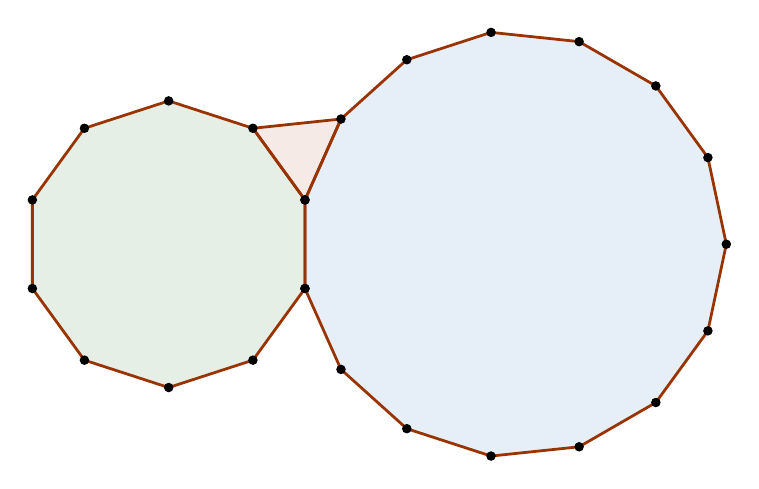
\begin{tikzpicture}[scale=.75]
\tkzSetUpLine[line width=1pt,color=black]
\tkzSetUpPoint[fill=black]

\tkzDefPoints{0/0/P0,0/1.5/P1,0/1.5/Q0,0/0/Q1}

\tkzDefRegPolygon[side,sides=10](P0,P1)

\tkzDefRegPolygon[side,sides=15,name=Q](Q0,Q1)

\tkzDefMidPoint(P1,P2) \tkzGetPoint{M1}
\tkzDefMidPoint(P2,P3) \tkzGetPoint{M2}
\tkzDefMidPoint(P3,P4) \tkzGetPoint{M3}
\tkzDefMidPoint(P4,P5) \tkzGetPoint{M4}
\tkzDefMidPoint(P5,P6) \tkzGetPoint{M5}
\tkzDefMidPoint(P6,P7) \tkzGetPoint{M6}
\tkzDefMidPoint(P7,P8) \tkzGetPoint{M7}
\tkzDefMidPoint(P8,P9) \tkzGetPoint{M8}
\tkzDefMidPoint(P9,P10) \tkzGetPoint{M9}
\tkzDefMidPoint(P10,P1) \tkzGetPoint{M10}


\tkzFillPolygon[fill=AngleClr,fill opacity=0.1](P1,P2,P3,P4,P5,P6,P7,P8,P9,P10)
\tkzFillPolygon[fill=BlueClr,fill opacity=0.1](Q1,Q2,Q3,Q4,Q5,Q6,Q7,Q8,Q9,Q10,Q11,Q12,Q13,Q14,Q15)

\tkzDefCircle[circum](P1,P2,P3) \tkzGetPoint{O}

\tkzFillPolygon[fill=ShapeClr,fill opacity=0.1](P3,P2,Q15)

\tkzDrawPolygon[color=ShapeClr](P1,P2,P3,P4,P5,P6,P7,P8,P9,P10)
\tkzDrawPolygon[color=ShapeClr](Q1,Q2,Q3,Q4,Q5,Q6,Q7,Q8,Q9,Q10,Q11,Q12,Q13,Q14,Q15)
\tkzDrawPolygon[color=ShapeClr](P3,P2,Q15)
\tkzDrawPoints[size=3](P1,P2,P3,P4,P5,P6,P7,P8,P9,P10)
\tkzDrawPoints[size=3](Q1,Q2,Q3,Q4,Q5,Q6,Q7,Q8,Q9,Q10,Q11,Q12,Q13,Q14,Q15)


\end{tikzpicture}

\end{document}
